\appendix

\renewcommand{\thefigure}{A.\arabic{figure}}
\setcounter{figure}{0}
\renewcommand{\thetable}{A.\arabic{table}}
\setcounter{table}{0}

\chapter{Appendix}
\section*{}

\begin{figure}[h!]
    \centering
    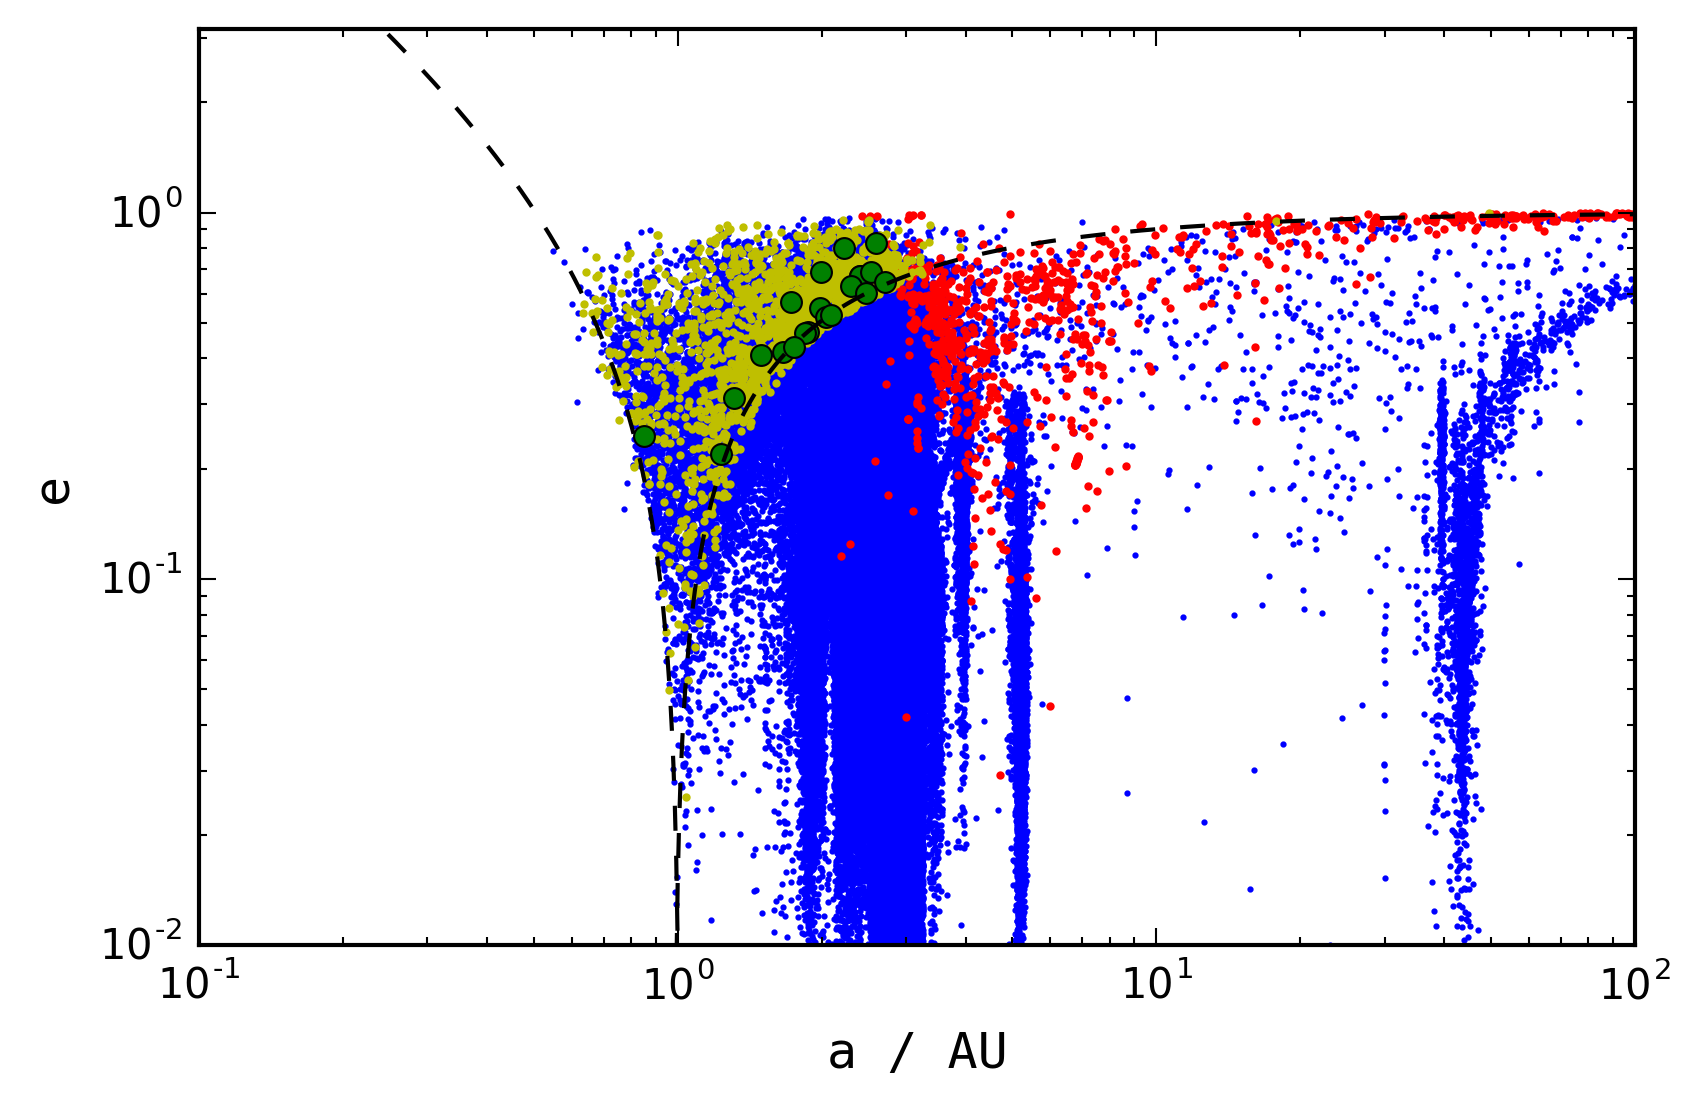
\includegraphics{losscone.png}
    \caption[Earth's loss cone]{Semi-major axes vs eccentricities of observed asteroids (blue), comets (red) and potentially hazardous asteroids (yellow). Data sourced from the IAU MPC. Meteorites with pre-impact orbits determined by \cite{doi:10.1093/mnras/stv378} are plotted as green circles. The Earth aphelion and perihelion are plotted as dashed lines.}
    \label{fig:loss_cone}
\end{figure}

\begin{figure}[h!]
    \centering
    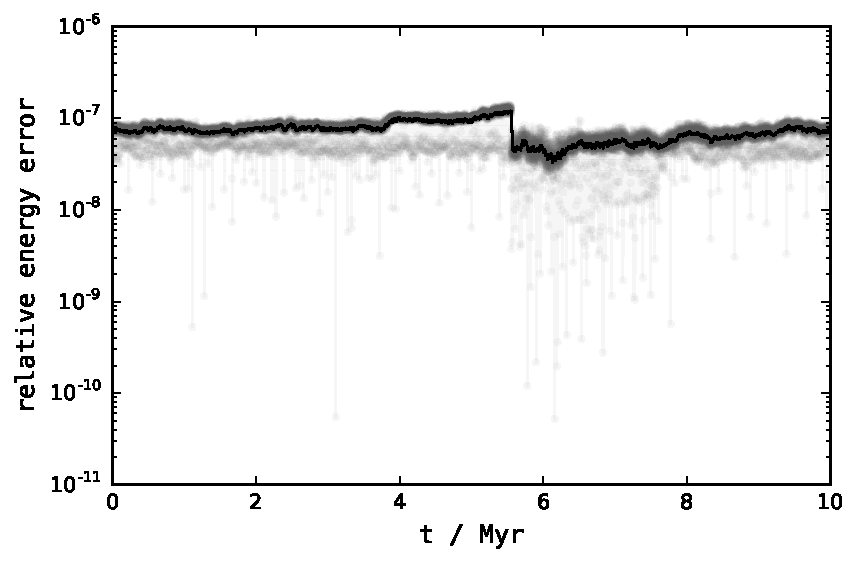
\includegraphics{figures/error.pdf}
    \caption[Simulation error]{Relative energy error over time. Black line shows the moving average of all the simulation runs.}
    \label{fig:loss_cone}
\end{figure}


\begin{sidewaystable}
\caption[Initial conditions]{Initial conditions of the solar system as of 01-12-2017 12:00 UTC. Data sourced from NASA JPL Horizons database.}\vspace{3ex}
\label{table:init_con}
\begin{tabular}{llllllll} \toprule \toprule
\multicolumn{1}{c}{Object} & \multicolumn{1}{c}{Mass / $M_{\odot}$} & \multicolumn{1}{c}{$x$ / AU} & \multicolumn{1}{c}{$y$ / AU} & \multicolumn{1}{c}{$z$ / AU} & \multicolumn{1}{c}{$v_x$ / AU$\;$yr$^{-1}$}& \multicolumn{1}{c}{$v_y$  / AU$\;$yr$^{-1}$}& \multicolumn{1}{c}{$v_z$  / AU$\;$yr$^{-1}$}\\ \midrule
Sun & 1.000E+00 & 1.977E-03 & 5.974E-03 & -1.244E-04 & -2.047E-03 & 1.909E-03 & 4.906E-05 \\
Mercury & 1.660E-07 & 3.336E-01 & 8.143E-02 & -2.438E-02 & -4.270E+00 & 1.048E+01 & 1.248E+00 \\
Venus & 2.448E-06 & -4.901E-01 & -5.244E-01 & 2.100E-02 & 5.361E+00 & -5.058E+00 & -3.788E-01 \\
Earth-Moon system & 3.040E-06 & 3.515E-01 & 9.280E-01 & -1.647E-04 & -5.980E+00 & 2.206E+00 & -1.903E-05 \\
Mars & 3.227E-07 & -1.649E+00 & 3.172E-03 & 4.033E-02 & 1.975E-01 & -4.673E+00 & -1.028E-01 \\
Jupiter & 9.548E-04 & -4.396E+00 & -3.189E+00 & 1.115E-01 & 1.586E+00 & -2.100E+00 & -2.676E-02 \\
Saturn & 2.859E-04 & -1.129E-01 & -1.006E+01 & 1.793E-01 & 1.926E+00 & -2.944E-02 & -7.613E-02 \\
Uranus & 4.366E-05 & 1.778E+01 & 8.962E+00 & -1.970E-01 & -6.572E-01 & 1.216E+00 & 1.303E-02 \\
Neptune & 5.151E-05 & 2.865E+01 & -8.684E+00 & -4.815E-01 & 3.249E-01 & 1.104E+00 & -3.022E-02 \\
\bottomrule
\end{tabular}
\end{sidewaystable}
